\documentclass[12pt]{article}
\usepackage[a4paper,left=2cm, right=2cm, top=2cm, bottom=2cm]{geometry}
\usepackage{amssymb}
\usepackage{amsmath,mathtools}
\usepackage{relsize}
\usepackage{epsfig,graphicx}
\usepackage{color}
\usepackage{tikz}
% \usepackage{subfigure}
\usepackage{hyperref}
\usepackage{algorithm}
\usepackage{algorithmic}
\usepackage{cite}
\usepackage{amsfonts}
\usepackage{textcomp}
\usepackage{xcolor}
\usepackage{multirow}
\usepackage{authblk}
\usepackage{subcaption}

\begin{document}

% \def\BibTeX{{\rm B\kern-.05em{\sc i\kern-.025em b}\kern-.08em
%     T\kern-.1667em\lower.7ex\hbox{E}\kern-.125emX}}

\title{Route Optimization For Waste Collection\\}

\author[1]{Marut Priyadarshi}
\author[2]{Meet Maratha}
\author[3]{Mohammad Anish}
\affil[1]{Department of Data Science Engineering, IISER Bhopal}
\affil[2]{Department of Data Science Engineering, IISER Bhopal}
\affil[3]{Department of Physics, IISER Bhopal}

\maketitle

\section{Introduction}
Waste collection is one of the most common yet one of the most integral systems present in all modern societies, helping maintain a sanitary environment across the urban landscape. And this system is going to become even more important as the global waste generation is set to increase with time. Global municipal solid waste generation levels, in the year 2012, were recorded to be 1.3 billion tonnes per year and this is expected to increase to 2.2 billion metric tonnes per year by the year 2025. According to data, the highest waste produced per capita is due to the wealthy countries (around 2.1 kg per day per capita.) whereas low-income countries have the lowest waste produced per capita (around 0.6 kg per day per capita).\cite{hoornweg2012waste}

In a study done about the costs of municipal waste collection for the city of Kragujevac, the annual costs of waste collection amount to nearly 14000 euros, which accounts for about 70\% of the total municipal solid waste costs \cite{boskovic2016calculating}. That was the case for a city with a population of around one hundred and fifty thousand people. For a larger city, the cost may be exponentially higher, owing to the complexity and challenges a larger population entails.

As seen, a lot of resources go into maintaining the waste collection system, which for the wealthy and more developed nations is not much of a problem, but for a resource constrained society, these costs may end being quite prohibitive, leading to insufficient waste collection and resulting in a decline of sanitation and public health.\cite{hamer2003solid}. Furthermore, due to insufficient funding, the gap in the supply of waste collection facilities and their demands may have to be met by manual waste pickers and thus endangering another group of people with health issues.\cite{gutberlet2017household}

Another secondary effect of inefficient waste collection systems is the emission of carbon dioxide, oxides of nitrogen and other gases and particulates from the collection vehicles, which are mostly run on diesel. These have a major hand in promoting global warming and other adverse weather phenomena such as acid rain. Studies have shown that these emissions can be significantly reduced by optimizing the collection routes so that the trucks have to traverse shorter distances \cite{apaydin2007route}. 

There is an abundance of literature addressing waste collection systems in developed countries, while the number of works pertaining to developing nations is scarce compared to it. Therefore, at this point, we have very little data regarding these systems or their implementation in resource constrained societies. As a result, we are focusing on the problem of reducing the cost of waste collection on on a technical level with an especial focus on resource constrained societies, which can be scaled and applied universally.

Vehicle route planning is the key to a good waste collection system, and it requires modeling a lot of components such as path optimization, consideration of available resources, spatiotemporal dynamics of waste volume at collection points and trucks, etc. A plethora of literature is present that addresses subsets of these components in the solution development. However, a holistic waste collection system must consider them simultaneously for any region. Such a study has not yet been reported in the literature. Hence, the on-ground implementation of the present approach is still very limited. This will have a significant impact on the operation costs and, eventually, on the environment. Moreover, the components and their interrelationships are very complex for resource constrained societies, and therefore pose altogether new challenges, requiring urgent attention of researchers.

To address the challenges stated above, we propose a waste collection framework for cities, with the objective to find the optimal routes for the available vehicle paths while considering the dynamic variations in the waste information at collection points and also that of the vehicles. The problem of finding the best path is formulated as an optimization problem and is solved using linear programming. The approach has an advantage over other traditional path planning approaches as it has wider applicability, is more interpretable, and maybe more efficient and robust.

The paper has the following major contributions:
\begin{itemize}
\item Analysis of truck availability in study regions on waste collection, to demonstrate the total coverage.
\item Consideration of quantitively simulated dynamic waste levels for truck and
collection bins for realistic outcomes.
\item Detailed sensitivity analysis of various parameters affecting selection of the best path.
\end{itemize}

\section{Related Studies:}

There has been a multitude of papers that have worked on different aspects of waste collection, such as the costs, route optimization and landfill and depot optimal locations. But, by far, the most common topic of work in this area has been route optimization and, in recent years, Internet of Things (IoT) enabled smart sustainable designs for the waste management systems. It poses a lot of challenges and there are a lot of possible solutions and methods that may be suitable for different cases. 

In one paper \cite{kulcar1996optimizing}, the author focuses on the best location for the construction of a landfill that would result in the shortest collection routes when linked with the currently existing routes and depots. The paper also compares the running costs of different modes of waste transport, such as trains, ships and by road. It was useful in providing a picture of the costs associated with the system, it didn't focus on optimizing the routes that the waste collection was done. Moreover, it was set in Brussels, a highly developed city. In a similar vein, Rathore et al. \cite{rathore2020location} focuses on formulating a mathematical model for finding the optimal places to allocate bins in the Indian city of Bilaspur. While it aims towards the similar goal of waste collection optimization, furthermore in a developing country, the method is different from our intended goal

Many papers utilize pre-existing solvers or software to compute the optimized routes and use the results to compare them to other algorithms or observe the effects the optimized routes bring to the current system. In the case of one paper \cite{karadimas2008routing}, the sole focus of the paper is on route optimization. However, it only applies ant colony system and the route optimizer for the software ArcGIS Network Analyst to get the optimal route for non-real time data and compares the efficiencies of the two methods. Moreover it focuses on Athens, another developed city, and even then on only one prefecture of it. Similarly, Chaudhary et al \cite{chaudhary2019gis} have utilized ArcGIS Network Analyst software to calculate optimal routes for waste collection, this time in the city of Allahabad. This lies closer to our goal of route optimization for more resource constrained societies and while it is an extensive application of optimization process utilizing the real-life data from the city, it still only utilizes a pre-existing algorithm along with fixed unchanging datapoints to calculate the collection routes, which our work seeks to expand upon. Another paper \cite{amal2018sga} uses the route optimization solver of GIS software ArcGIS (which itself utilizes Dijkstra algorthm) to calculate a pool of routes which, in turn, feeds the genetic algorithm to iteratively arrive at the optimal routes for the waste collection vehicles.

In their paper, Simonetto and Borenstein \cite{de2007decision}, they used linear programming to formulate a function for route optimization via minimization of cost coupled with a heuristic developed by Renaud and Boctor \cite{renaud2002sweep} in order to bring down the computation time (at that time) to reasonable levels. Similarly, in this paper \cite{hannan2020waste}, the authors have used linear programming combined with smart bins to find optimal waste collection routes that remove the inefficiency that is associated with formulating a route that visits all nodes, regardless of its fill status. However, as it was a paper focused on the algorithmic part of the problem, they used purely simulated data, void of any real world analogue and only factored in the euclidian distances between the nodes. Asefi et al \cite{asefi2019mathematical} uses a mixed-integer linear programming model to minimize costs and uses two different meta heuristic approaches to deal with the non-deterministic polynomial-time hardness of the waste collection problem. This model is then applied to a case study in the city of Tehran, Iran. 

In other papers utilizing smart bins, Akhtar \cite{akhtar2017backtracking} utilizes new population based meta heuristic backtracking search optimization, developed by Civicioglu \cite{civicioglu2013backtracking}, to calculate optimal routes for collection vehicles. Its main feature is its simplicity as it has only one control parameter. It is also a highly theoretical work and focuses mainly on the mathematical aspects of the problem and not its real-life application. Al-Refaie et al \cite{al2021optimization} takes a different approach and focuses instead on distributing the collection points into optimal clusters so that the collection efficiency of the vehicles can be maximized.

Papers like Lozano et al \cite{lozano2018smart} and later Baldo et al \cite{baldo2021multi}, Vishnu et al \cite{vishnu2021iot} use smart bins, but the focus of these papers are the smart bins themselves, their engineering aspect and case studies involving them, along with constructing a system centered around technology which automates a lot of the tasks involved in the whole process of waste collection and management. The optimization part is left to pre-existing solving algorithms.

Smart bins have also been discussed in a more theoretical aspect, utilizing IoT technology in other studies such as Abdullah et al \cite{abdullah2018iot}, Ali et al \cite{ali2020iot}, Al-Masri et al \cite{al2018serverless} and Chaudhari and Bhole \cite{chaudhari2018solid}. They have touched upon smart bins as parts of a sustainable smart city architecture and different ways that they may be utilized, along with supporting subsystems. It should be noted that the above-cited literature is in no way an exhaustive list of literature utilizing IoT or smart bins, and merely provides a general idea of the works using it.

In our paper, our main priority is to create a model for route optimization that is suitable for a resource constrained city, yet is general enough to be scaled to fit more developed societies. Moreover, our model works with real time data, capable of adapting to new data and calculating new routes based on changing information, and that information is gained through another concept used in our paper called smart bins. This paper also seeks to keep the simulated data as close the real life situations as possible so that the gap between theory and implementation would be minimal.

Our model integrates the concept of smart bins with the optimization algorithm. As mentioned before, smart bins are simply bins that are connected to the internet and provide real time data on how full they are. This data is used by the model to calculate new optimal routes for the collection vehicles after a specified time interval, based on the real-time locations of the vehicles. The engineering and construction aspects of the smart bins are outside the scope of this paper, however other works have delved into much more detail on this problem.

\section{Problem Formulation}

In route optimization, we need objectives that we either need to maximize or minimize, according to our goals, and then make an objective function which then is solved to give us the best route. 

In our problem, our two main objectives are:
\begin{itemize}
    \item Minimize the distance travelled by the collection vehicles
    \item Maximize the waste collected through the collection run
\end{itemize}

With this we can formulate our base objective function to be:

\begin{equation}\label{eq1}
    Obj(minimize)=\sum_{i,j \forall A} w_1 X_{ij} C_{ij} - w_2 Y_i f_i * BT
\end{equation}

Here, $X_{ij}$ is a binary variable that can only take the values 0 or 1, based on the fact if a truck took a route from i to j. $C_{ij}$ is the cost, or the distance travelled when moving from i to j. $Y_{i}$ is another binary variable that indicates if waste from node i has been collected or not. $BT$ is the conversion factor of how much would the waste from a node would fill up a truck collecting it. $f_i$ represents the fill ratio (the percentage of how full the bin is) of the bin, its value being 0 and 1. 0 meaning it's empty and 1 meaning it is full. $w_1$ and $w_2$ are the weights associated with distance travelled and waste collected, respectively, to determine which attribute of waste collection should have the higher priority and by how much. 

We have divided this problem into two cases.
\begin{itemize}
    \item Static: In this case, the optimal route calculation is done only once, in the beginning of a collection run, based on the fill ratios of the bins. The values are not updated during the time of the run.
    \item Real-time: In this case, the fill ratios are updated throughout the run after fixed intervals. After each updation, new optimal routes are calculated to account for the new data according to our objective function.
\end{itemize}

For the objective function to fully represent our problem, we need to add constraints.

\textbf{First, for the static case:}
\begin{equation}\label{eq2}
    \sum_{j\in N} X_{0 j}=1
\end{equation}
\begin{equation}\label{eq3}
    \sum_{j\in N} X_{j0}=1
\end{equation}
Node 0 is assigned to be the depot, the start and the end point of every collection run. Eq \eqref{eq2} and Eq \eqref{eq3} ensure that all runs start and end from node 0.
\begin{equation}\label{eq4}
    \sum_{i\in N}\sum_{j\in V, J\ne i} X_{ji}=1
\end{equation}
\begin{equation}\label{eq5}
    \sum_{i\in N}\sum_{j\in V, J\ne i} X_{ij}=1
\end{equation}
N is the set of all nodes, V is the set of all the nodes excluding node 0. Eq \eqref{eq4}
and Eq \eqref{eq5} specify that visited nodes are not visited again.
\begin{equation}\label{eq6}
    \sum_{i\in N}{y_{i}f_i*BT}\le100
\end{equation}
Eq\eqref{eq6} ensures that any truck never goes past being 100\% full.
If
$$ X_{ij}=1$$
then
\begin{equation}\label{eq7}
    u_1+f_1*BT =u_j
\end{equation}
for 
$$ \forall i,j \in A$$
$$ i,j\ne 0$$
This constraint (Eq \eqref{eq7}) ensures that if a truck goes on an arc from node i to node j, the amount of waste is continuous, ie. the waste in the truck at node j is the sum of the waste at node i and the waste collected in the route i to j. And the value of the waste inside the truck is updated at node j.
\begin{equation}\label{eq8}
    u_i\ge f_i*BT
\end{equation}
$$  \forall i\in N$$
Eq\eqref{eq8} simply ensures that the amount of waste in a truck after traversing an arc from i to j must always be greater or equal to the waste before traversing the path.
\begin{equation}\label{eq9}
    u_1\le100
\end{equation}
$$\forall i\in N $$
Eq\eqref{eq9} ensures that the value of the waste at the truck at any given node does not exceed 100\% of its capacity.

\textbf{Now for the real-time case:}

The objective functions remains the same, only a few more variables are added to the constraints. the subscript 'st' denotes the starting node at the start of the calucations after the given time interval. $T_i$ denotes the percentage of the truck that is full at a given node i
\begin{equation}\label{eq10}
    \sum_{j\in N}x_{st,j}=1
\end{equation}
\begin{equation}\label{eq11}
    \sum_{j\in N}x_{j,st}=1
\end{equation}
Like the static case, Eq (\ref{eq10}) and Eq (\ref{eq11}) ensure the looping of the route, except here, since the calculations are made multiple times the value of the starting node for each calculation changes.
\begin{equation}\label{eq12}
    \sum_{i\in N}Y_i f_i* BT\le100
\end{equation}
Eq \eqref{eq12} ensures that the truck will only collect waste from a node if the total sum of the waste collected by it on the run is less than its maximum capacity.
If
$$X_{ij}=1$$
Then
\begin{equation}\label{eq13}
    u_i+f_1*BT=u_j
\end{equation}
$$\forall i,j\in A$$
$$i,j\ne 0 $$
$$ i,j \ne st $$
This is the same as in the case of static optimization, where the continuity of the waste amount is maintained and updated as the truck exits an arc of a route.
\begin{equation}\label{eq14}
    u_i\le 100 - T_i
\end{equation}
$$\forall i \in N $$
This constraint in Eq \eqref{eq14} ensures that the fill ratio at each node will be less than or equal to 100- fill ratio before that node.

With this, we have formulated our problem and now we can move on to implementing and calculating the solution for our problem

\section{Case Studies and Empirical Results}

\subsection{Data Preparation}

We have used a set of randomly selected points in the city of Chandigarh as the collection points that the collection vehicles have to travel to. The random bin locations were generated using QGIS function that generates random points inside a polygon, which in our case was the entire city. Then we divided the points into a certain number of wards, in our case: three, which depend on the number of vehicles that are available for the job. The wards were assigned by using K-Means Clustering algorithm by allotting the nodes into different clusters.

Now, since we are using the concept of smart bins, we also had to simulate their function. While running the optimization process, each individual bin is randomly assigned a value between 0 and 1 to denote how full the bin is. This value will be one of the parameters during the optimization process.

Next, we use another QGIS function called 'shortestpathtopoint' to calculate the distance between all points in the set, subject to the heuristic that all streets are undirectional, meaning all paths measure the same both ways and that a truck assigned to one ward will only collect from bins in its own ward.

\subsection{Implementation}

Since our objective function is a linear programming optimization problem, we have used gurobipy solver to solve our problem subject to the constraints given for each case.

For our nodes, considering Chadigarh's size and the amount of waste generated \cite{ravindra2015system}, we generated 300 collection points for our vehicles using QGIS. The data had to be scaled down for the sake of computation. We used the optimize function of gurobipy to solve our objective function subject to different restrictions and parameters.

Our objective function has two main objectives, maximizing waste collection and minimizing the distance travelled. In order to decide the relative importance of each objective, we have attached weights to both of them. To get the values of the weights $w_1$ and $w_2$, we solved the optimization problem with different weights, changing the weights in increments of 0.1 plotted a graph of the value of the objective function vs the weight and picked the weights which gave us the highest overall values for the objective function.       

In the route optimization process, we keep track of a few things such as the nodes visited, the nodes that are yet to be visited, which arcs in a route are selected, making sure the routes are continuous. Since we are using smart bins we only consider those nodes for the route calculation that are full beyond a certain threshold of its capacity. Then in the case of static optimization, one route is calculated that gives us the most optimal path for waste collection for that run.

In the real-time case, there are many more factors to consider, as the values for the nodes are being updated in real time, even while the truck is doing its collection run. If the time interval comes to pass when the truck is in between nodes, the program assumes the truck completed its current arc and considers the next node as the starting point of the new route calculation. That node is then automatically added to the visited nodes list so that it is not factored in the next calculation.

For our average case simulation, the fill ratios for the smart bins are decided randomly, therefore some nodes do not need to be visited for that run.

Our algorithm is based on one single waste collection run per day, to show the resource constraint. But since we also intend for the algorithm to be scalable for a place where resources are not a problem and multiple trucks can be allotted for waste collection, we also have implemented a case where multiple trucks are allotted to run within one ward so that most of the nodes are able to be covered.
\subsection{Execution case studies}
\subsubsection*{Case 1: Weight Analysis}
In order to find the best pair of weights that will give us the best results, ie. the minimum value of the objective function, we need to take different weights, plug them into the objective function and plot the resulting graph (Figure \ref{fig1}). It shows the change in the objective function values for the iterated weights. The lowest point of this graph would give us the optimal weight. Since we want the relative importance of the two objectives, the total sum of the weights is equal to one, thus getting one weight means automatically getting the other.

\begin{figure}[h]
    \centering
    \begin{subfigure}{0.5\textwidth}
        \centering
        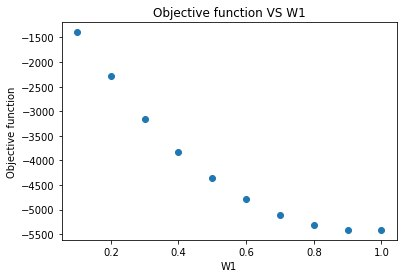
\includegraphics[width=\linewidth]{weight_analysis_w1.jpg}
        \caption{Obj vs $w_1$}\label{figw1}
    \end{subfigure}%
    \begin{subfigure}{0.5\textwidth}
        \centering
        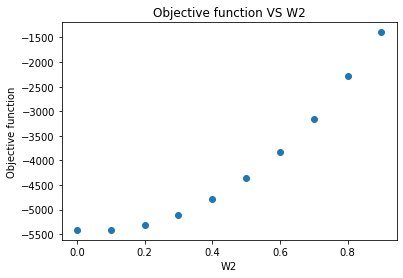
\includegraphics[width=\linewidth]{weight_analysis_w2.jpg}
        \caption{Obj vs $w_2$}\label{figw2}
    \end{subfigure}
    \caption{Weight Analysis}
    \label{fig1}
\end{figure}

We can see here that for the optimal results, the $w_1$ should be equal to 0.9 and $w_2$ equal to 0.1. This means that our optimization procedure should mainly focus on minimizing the distance and to a small extent maximizing the waste collected.

Now, we have the two cases for which we have solved the objective function for the optimal solution. For the sake of calculations, the maximum capacity of a truck is 1000 kgs of waste, and the maximum capacity of one smart bin is 100 kgs.

\subsubsection*{Case 2: Real-time, restricted}
In this case, the optimal routes will be calculated in real time after a recurring interval of time, but with limited resources which, in this case, are the trucks. We used 1, 2, 3, and 4 trucks per ward and comapared their performances. The weights, as calculated earlier, for distance minimization is taken as 0.9 and waste collection maximization is taken as 0.1

The following Table \ref{tab1} summaraizes the data obtained from realtime restricted optimization of routes where waste is calculated in kilograms and distance traveled in kilometres.
\begin{table}[H]
    \centering
    \caption{Data for the realtime restricted case} \label{tab1}
    \vspace*{0.3cm}
    \begin{tabular}{|c|c|c|c|c|c|c|}
        \hline \multirow{2}{*}{Case} & \multicolumn{2}{c|}{Ward 1} & \multicolumn{2}{c|}{Ward 2} & \multicolumn{2}{c|}{Ward 3}\\
        \cline{2-7}& Waste (Kg)  & Distance (Km) & Waste (Kg) & Distance (Km) & Waste (Kg) & Distance (Km)\\ 
        \hline \textit{1 Truck} & 994.55 & $67.8$ & 999.8 & $54.6$ & 998.51 & $50.2$ \\
        \hline \textit{2 Trucks} & 1988.6 & $144.6$ & 1994.74 & $191.2$ & 1990.86 & $210.4$ \\
        \hline \textit{3 Trucks} & 2981.16 & $188.7$ & 2982.81 & $255.01$ & 2983.33 & $247.04$ \\
        \hline \textit{4 Trucks} & 3974.77 & $198.1$ & 3972.95 & $224.4$ & 3978.04 & $218.5$ \\
        \hline
    \end{tabular}
\end{table}

We observe the case of 4 trucks per ward to determine whether it is sufficient to satisfy the waste collection demand of the city. Table \ref{tab3} summarizes the data obtained from running the algorithm with this setup.
\begin{table}[H]
    \centering
    \caption{ Data for 4 trucks per ward} \label{tab2}
    \vspace*{0.3cm}
    \begin{tabular}{|c|c|c|c|c|c|}
        \hline Ward & Truck & Waste (Kg) & Distance (Km) & Waste/Distance & Percent collected \\
        \hline \multirow{4}{*}{Ward 1} & Truck 1 & 987.94& 48.7 &0.0024  &17.8947\% \\
        \cline{2-6}& Truck 2 &999.97&32.1&0.0014&17.8947\%\\        
        \cline{2-6}& Truck 3 &995.37&75.2&0.0023&25.2632\%\\        
        \cline{2-6}& Truck 4 &991.49&42.2&0.0015&16.8421\%\\
        \hline & & & &\textbf{Total:} &\textbf{77.8947\%}\\
        \hline \multirow{4}{*}{Ward 2} & Truck 1 &997.93 &41.6  & 0.0023  &13.5135\% \\
        \cline{2-6}& Truck 2 &987.59&72.9&0.0014&16.2162\%\\        
        \cline{2-6}& Truck 3 &999.16&43.9&0.0023&12.6126\%\\        
        \cline{2-6}& Truck 4 &988.28&65.9&0.0015&15.3153\%\\
        \hline & & & &\textbf{Total:} &\textbf{57.6576\%}\\     
        \hline \multirow{4}{*}{Ward 3} & Truck 1 &999.25  &63.4  &0.0016  &20.2128\% \\
        \cline{2-6}& Truck 2 &999.96&44.8&0.0022&19.1489\%\\        
        \cline{2-6}& Truck 3 &991.13&50.7&0.002&19.1489\%\\        
        \cline{2-6}& Truck 4 &987.69&59.7&0.0017&19.1489\%\\
        \hline & & & &\textbf{Total:} &\textbf{77.6595\%}\\
        \hline      
    \end{tabular}
\end{table}

We can infer from the above data that the number of trucks falls just short of being able to satisfactorily able to cover most of the city's bins. It is only able to cover, on an average, 70\% of the total number of bins that need to be collected.

\subsubsection*{Case 3: Real-time, unrestricted}

In this case, we want to see the results of route optimization if the resources were not constrained and there were enough, in our case, trucks to cover the waste collection demands at a satisfactory level. From the previous case, we saw that 4 trucks per ward fell just short of being enough, so for this case, we raised the number of trucks to 5 per ward. Table \ref{tab3} summarizes the data obtained from this case.

\begin{table}[H]
    \centering
    \caption{ Data for 5 trucks per ward} \label{tab3}
    \vspace*{0.3cm}
    \begin{tabular}{|c|c|c|c|c|c|}
        \hline Ward & Truck & Waste (Kg) & Distance (Km) & Waste/Distance & Percent collected \\
        \hline \multirow{4}{*}{Ward 1} & Truck 1 &997.75  &49.8  &0.002  &18.9474 \\
        \cline{2-6}& Truck 2 &997.66&27.7&0.0036&16.8421\%\\        
        \cline{2-6}& Truck 3 &984.55&73.0&0.0013&21.0526\%\\        
        \cline{2-6}& Truck 4 &984.62&50.8&0.0019&17.8947\%\\
        \cline{2-6}& Truck 5 &980.61&97.8&0.001&23.1579\%\\
        \hline &\textbf{Total:} &\textbf{4945.2004} &\textbf{299.09} &- &\textbf{97.8947\%}\\
        \hline \multirow{4}{*}{Ward 2} & Truck 1 &999.19  &52.7  &0.0019  &14.4144 \\
        \cline{2-6}& Truck 2 &999.31&72.0&0.0014&15.3153\%\\        
        \cline{2-6}& Truck 3 &991.88&51.5&0.0019&15.3153\%\\        
        \cline{2-6}& Truck 4 &992.17&85.2&0.0012&18.9189\%\\      
        \cline{2-6}& Truck 5 &996.02&113.1&0.0009&26.1261\%\\
        \hline &\textbf{Total:} &\textbf{4978.5775} &\textbf{374.6} &- &\textbf{90.09\%}\\     
        \hline \multirow{4}{*}{Ward 3} & Truck 1 &998.91  &64.9  &0.0015  &18.0851 \\
        \cline{2-6}& Truck 2 &995.87&49.1&0.002&19.1489\%\\        
        \cline{2-6}& Truck 3 &997.85&43.9&0.0023&18.0851\%\\        
        \cline{2-6}& Truck 4 &999.48&71.5&0.0014&20.2128\%\\
        \cline{2-6}& Truck 5 &992.29&103.2&0.001&19.1489\%\\
        \hline &\textbf{Total:} &\textbf{4984.3948} &\textbf{332.7}&- &\textbf{94.6808\%}\\
        \hline      
    \end{tabular}
\end{table}

\begin{figure}[H]
    \centering
    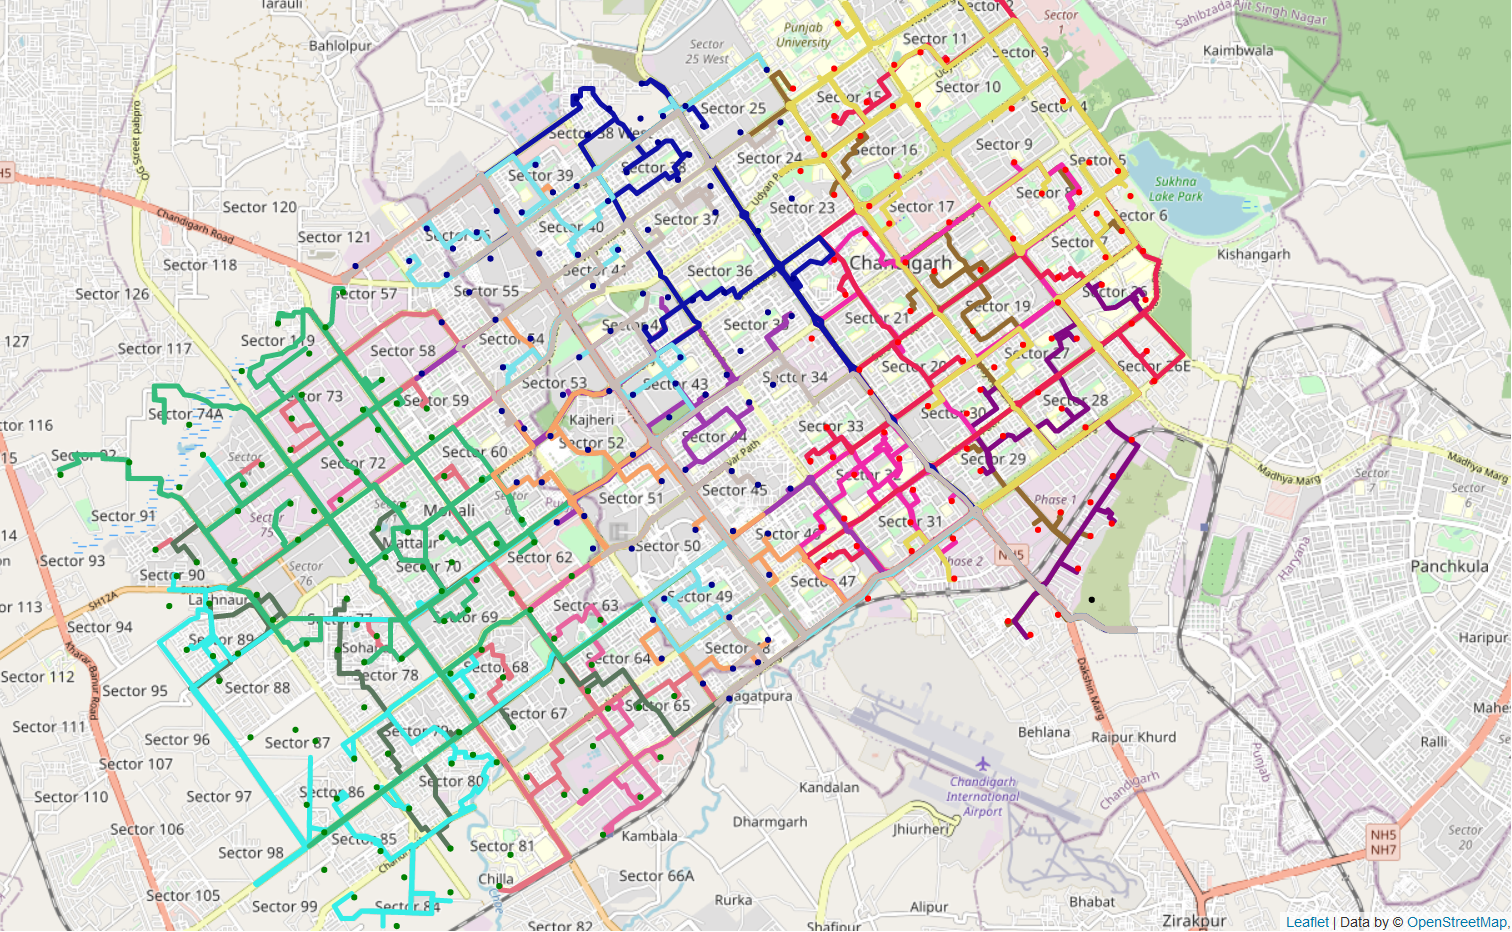
\includegraphics[scale=0.4]{Dynamic5trucks.png}
    \caption{Realtime Unrestricted}\label{fig2}
\end{figure}

From this data, we can easily observe that with 5 trucks per city ward, more than 90\% of the city's bins get covered, and with a similar procedure, more trucks can be added for even more efficient collection. While the total distance is increased, it is a direct result of having more trucks running at the same time, and since most of the bins are being collected, some trucks need to traverse outlying regions to cover the remaining bins. This is visualised in Figure \ref{fig2} where we have plotted the optimized routes dictated by the objective function.

\subsubsection*{Case 4: Impact of the number of trucks on total coverage.}

As expected from our previous cases, increasing the number of trucks available per ward leads to a more thorough collection of waste as shown in Table \ref{tab4} and represented graphically in Figure \ref{fig3}. Compared to case 2, where the number of trucks per ward was varied from 1 through 4, we can see a clear rise in the coverage of bins as we increase the number of trucks, concluding in the last and our best case of 5 trucks. Having more trucks at your disposal is a matter of resources, and for a resource constrained region, their availability of trucks may not be sufficient for the amount of waste generated which will, unless overcome by alternate methods such as multiple collection runs per vehicle, will lead to subpar waste collection, as shown by the data. However, those alternate methods are beyond the scope of the current work.
\begin{table}[H]
    \centering
    \caption{ Bins coverage in percent based on number of trucks per ward} \label{tab4}
    \vspace*{0.3cm}
    \begin{tabular}{|c|c|c|c|c|c|}
        \hline \multirow{2}{*}{Ward} & \multicolumn{5}{c|}{Number of trucks}\\
        \cline{2-6}& 1 Truck& 2 Truck& 3 Truck& 4 Truck& 5 Truck\\
        \hline \textit{Ward 1} & 11\%& 45.2632\%& 66.3158\%& 77.8947\%& 97.8947\%\\
        \hline \textit{Ward 2} &10.8108\%&36.9369\%&53.1531\%&57.6576\%&90.09\%\\
        \hline \textit{Ward 3} &11.7021\%&44.6808\%&61.7021\%&77.6595\%&94.6808\%\\
        \hline
    \end{tabular}
\end{table}


\begin{figure}[H]
    \centering
    \begin{subfigure}{0.5\textwidth}
        \centering
        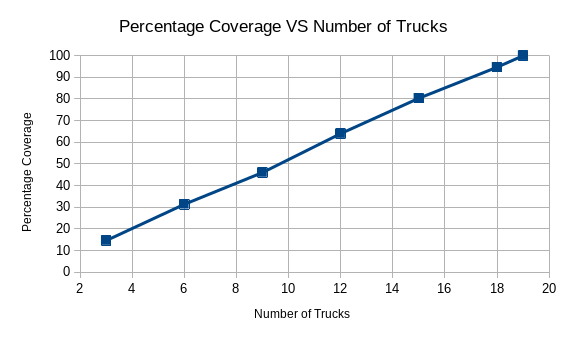
\includegraphics[width=\linewidth]{coverage_VS_number_of_trucks.png}
        \caption{For the entire city}\label{figc1}
    \end{subfigure}%
    \begin{subfigure}{0.5\textwidth}
        \centering
        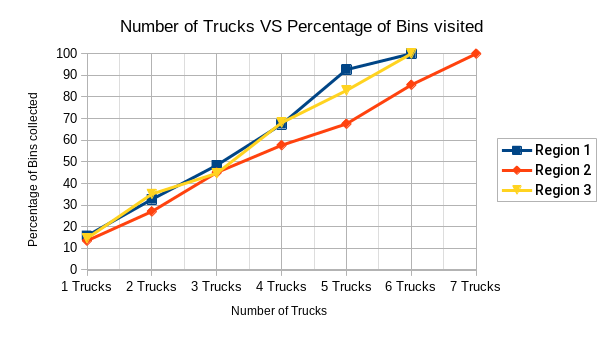
\includegraphics[width=\linewidth]{number_of_trucks_VS_bins_visited.png}
        \caption{In terms of wards}\label{figc2}
    \end{subfigure}
    \caption{Effect of number of trucks on bin coverage}
    \label{fig3}
\end{figure}

\subsubsection*{Case 5: Comparison of real-time with static route calculation}

While our main method of route calculation works in real time by getting new fill values from the smart bins throughout the collection run and calculates new best routes based on the truck's current position in real time, there is another, more simpler method that trades off the reliability and adaptability of the real-time method for faster computational time and slightly more efficient routes.

To compare the two methods, for the sake of simplicity, we will use the 1 truck per ward case from case 2 and compare it to the static method by applying it to the same 1 truck per ward case. The comparison is represented in Table \ref{tab5}

\begin{table}[H]
    \centering
    \caption{Comparison of static and real-time optimization performance} \label{tab5}
    \vspace*{0.3cm}
    \begin{tabular}{|c|c|c|c|}
        \hline Case & Waste (Kg) & Distance (Km) & Percent Covered\\
        \hline \textit{Static}& 2999.32& 113.2 & 42.11\%\\
        \hline \textit{Real-Time}& 2992.85& 172.6& 34.09\%\\
        \hline
    \end{tabular}
\end{table}

Figure \ref{fig4} and Figure \ref{fig5} are the plots of the routes calculated by the static and the real-time optimization methods respectively.

\begin{figure}[H]
    \centering
    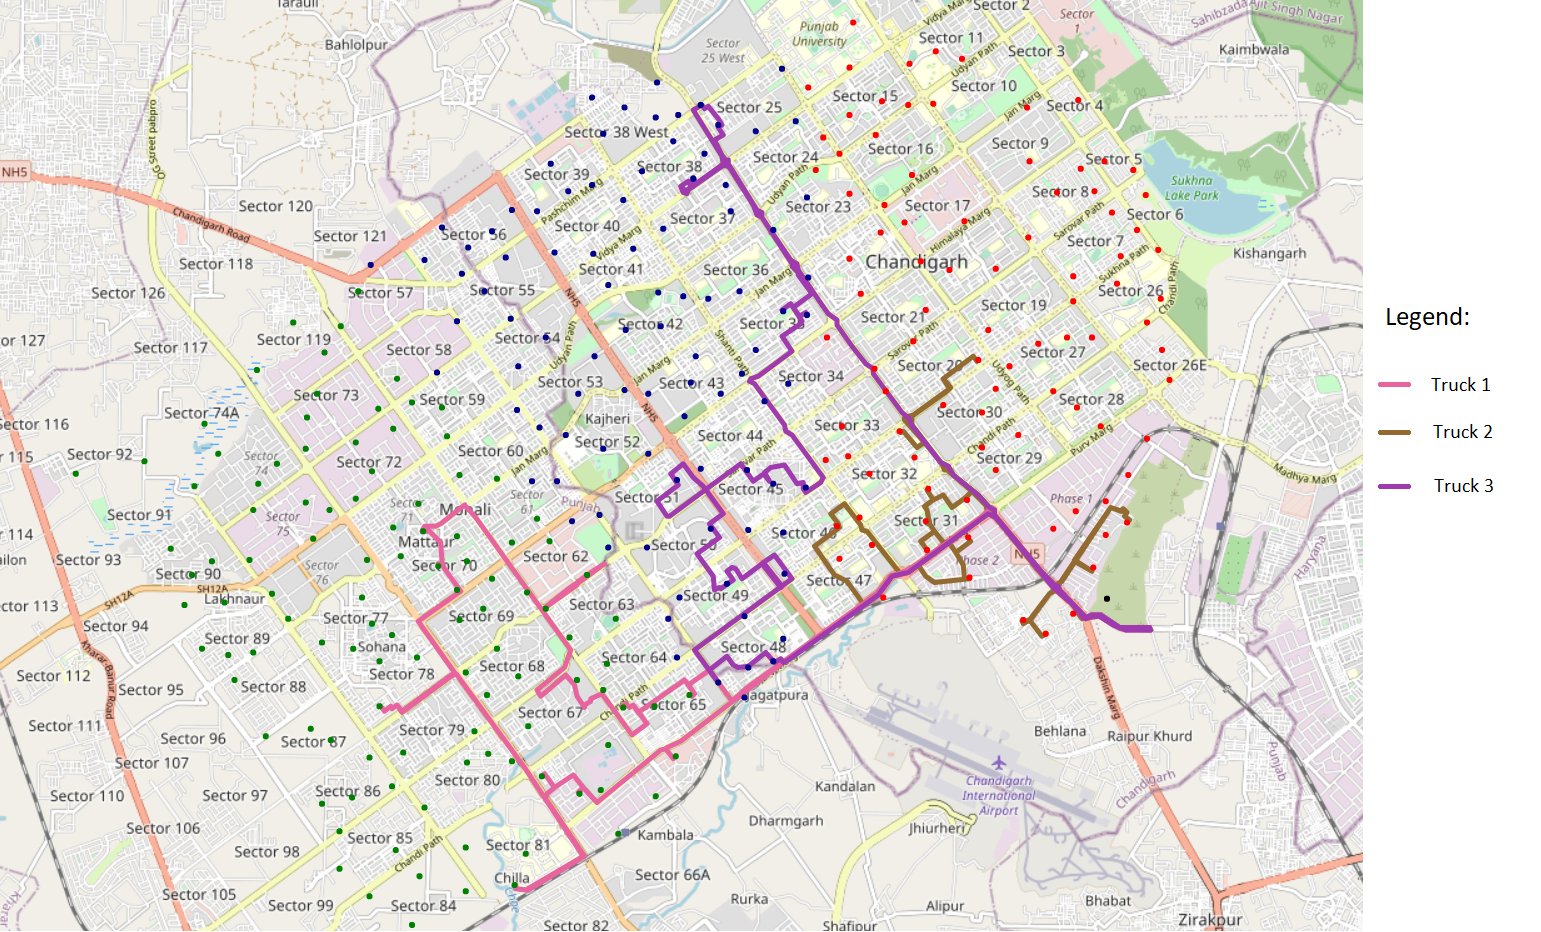
\includegraphics[scale=0.4]{Static1truck.png}
    \caption{Routes for 1 truck per ward as calculated by static optimization}\label{fig4}
\end{figure}
\begin{figure}[H]
    \centering
    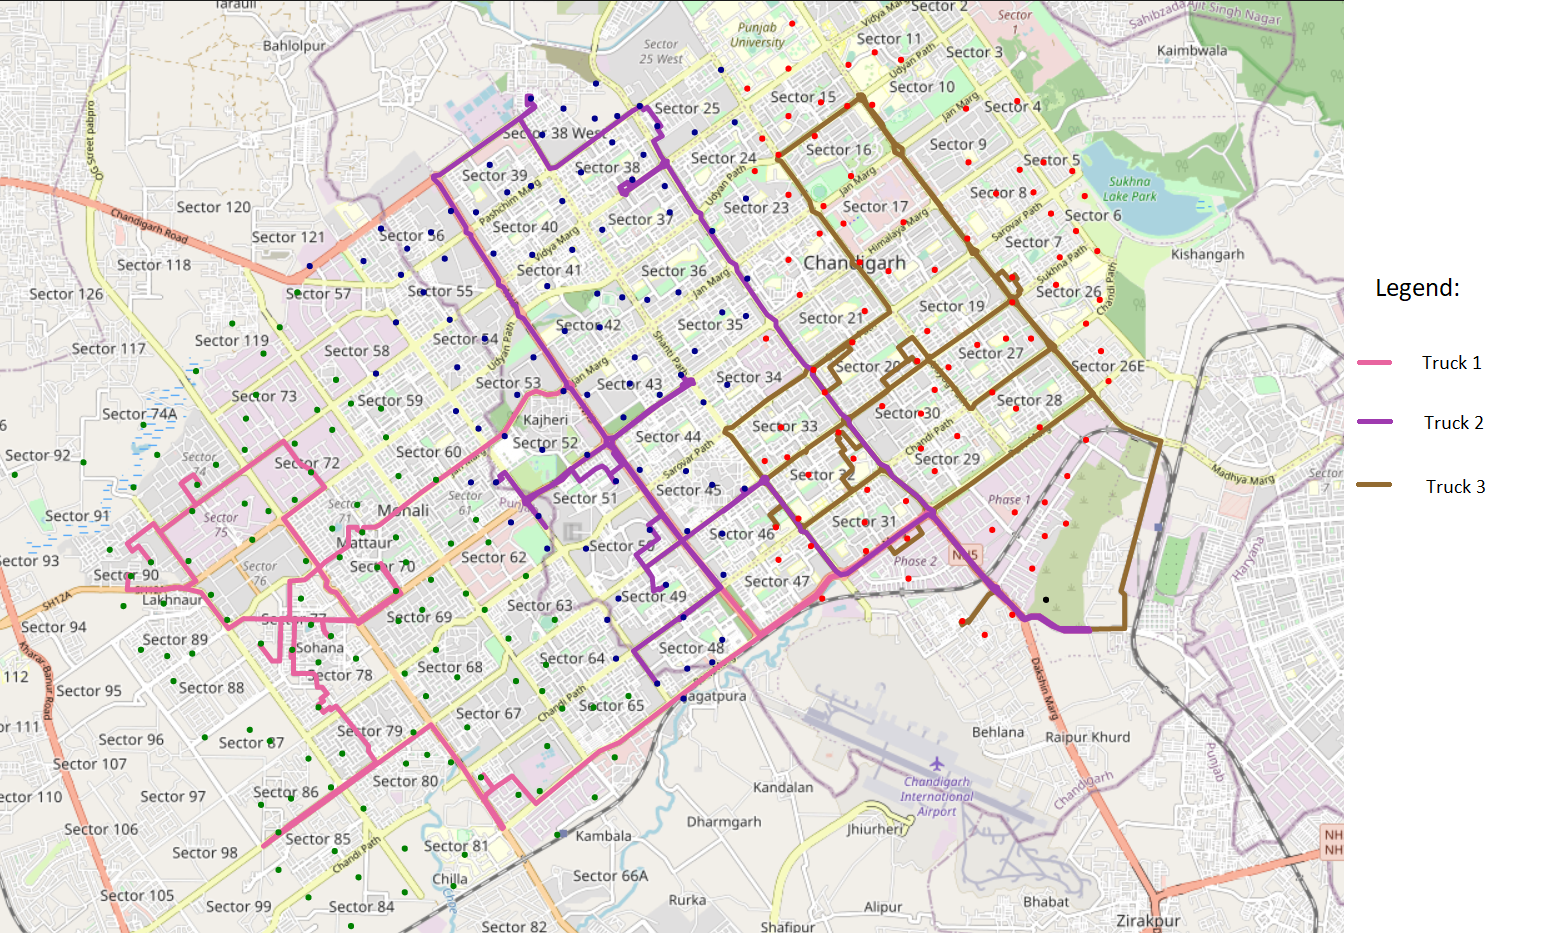
\includegraphics[scale=0.4]{Dynamic1truck.png}
    \caption{Routes for 1 truck per ward as calculated by real-time optimization}\label{fig5}
\end{figure}
We observe that the weight of the waste collected is nearly the same but the distance travelled by the trucks is smaller in the static case. This can be easily explained by the fact that, in essence, real-time method is just the static method applied repeatedly after certain intervals of time. Therefore, static gives one optimal route for the currently available data, but real-time has to do that each time the data is updated. It has to calculate new routes multiple times, even when the vehicle is already traversing the previous optimal route, and it also has to take the current position of the vehicle into consideration. This makes it inherently slightly more inefficient compared to the static method. 

This makes static optimization superior but only theoretically, because when applied in the real world, static has a lot of disadvantages that real-time solves, such as the adaptability. In the static case, there is no accounting for new data. The initial route is the only route. This, consequently, also makes it unreliable. Real-time method, on the other hand, accounts for new data and creates new optimal routes taking it into consideration, making it very adaptable and reliable. Since real-time is just a modified and iterated version of the static method, the difference in computational power required between the two methods is not large. 

Therefore, for real life applications, real-time method is the superior method as it is able to deal with non-deterministic events that are common for ground use and adapt to them, giving an uninterrupted and reliable result.


\section{Discussion and Policy Suggestions}
One of the most noticeable observations that can be derived from the results is the weights attached to the two objectives in the objective function. In this case, the distance traveled was computed to be the main factor which must be considered when solving the objective function for the optimal solution. The waste collected appears to be almost completely irrelevant in this case. While this may look like an anomaly, this is solely due to the fact that this is a resource constrained operation. The trucks  have to continue their runs until they are full. Therefore, in the end, the amount of waste collected will always be equal to the maximum capacity, hence rendering maximizing the waste collected objective irrelevant.

However, we must keep in mind that this will not always be the case. In a case where the resources, ie. the trucks are more than sufficient to cover the demand, the weight for the objective to maximize waste collected will be greater. The more is the resource greater than the requirement, the greater the weight of that objective will be.

We also observe that the distance travelled in the case of real-time optimization is greater than that of static one. It is due to the fact the optimal routes are calculated multiple times with different starting points based on the truck's current location. This makes the resultant route slightly more inefficient when compared to the initial calculation. This is an unavoidable effect of recalculating the routes and not a problem with the algorithm as the path that is already been travelled is not considered by the newly calculated route, hence the resultant route is longer than the initial optimal route

We have selected the city of Chandigarh as the base location for paper because while it is our goal to focus on resource constrained regions for route optimization for waste collection, we also want to make it general enough so that with a few tweaks, the same method can also be scaled to be used for more developed regions and cities. Chandigarh was found to be the most suitable choice as it is the perfect blend of the two goals that we have: it is a well-planned city and still retains some of the characteristics of a developing nation.

Our program, once the initial setup of the nodes and the distance between two nodes is done, can efficiently and quickly calculate the optimal route that should be followed by a collection vehicle, whether once per run or in real time. Unlike the currently used systems that are either controlled manually or use general GPS systems to do their collection runs, our process is capable of:
\begin{itemize}
    \item Vastly improved performance in terms of distance travelled
    \item Smart bins further reduce the distance travelled by removing the need to visit redundant nodes
    \item We have used linear programming which is a simple yet novel approach to this problem and it is not too mathematically complex
    \item Our program is able to calculate new paths according to new data in real-time which is much more flexible than the systems currently being used in most places
    \item We also calculated the effects of resource availability on the overall performance and can further suggest the minimum amount of resources that would be sufficient for the operation.
\end{itemize}

For real world application of this method, the suggested policy would be to first use the software to calculate the current capabilities of the resources that are available, then apply the algorithm to utilize those resources, namely trucks, to their maximum potential and efficiency. If needed, how much more resources are needed to sufficiently cover the city in question can also be calculated by the software, and the results can be used as data for the requisition request of more resources.

\section{Conclusion}
We have achieved most of our core goals of optimizing waste collection with a focus on resource constrained societies. We were able to devise a method to use the available resources as efficiently as possible and at the same time ensure that the method also remains viable in more developed regions if scaled accordingly. Yet there still were things that we were not able to implement in our current endeavour. 

In our process, we divide the total number of nodes into specific clusters depending upon the resources that we have. These clusters are called wards and in the current version, vehicles assigned to each cluster are completely independent of the points in another cluster, and will not collect from a node from another cluster even when it is more efficient to do so. 

These can be taken as goals for future forays into this field to overcome the current limitations of our work. Scopes for future development may focus on improving upon our works by integrating more detailed street data like street signs, one-way roads and using the additional parameters as factors to provide a more street accurate route tailored for a specific region.

Future works may also focus on the effects different sets of weights may have on the results of the objective function for different granular levels of resource constraint. In our current work, we have focused solely on the best weights for one specific case. So further research can be done to find a more concrete relationship between weights, results and resource availability. 

In our current method of real time route calculation, our algorithm does not consider the route already travelled when calculating the new routes for new data. This leads to some degree of inefficiency in the optimization process and is also a viable topic for further work in this field.
\bibliographystyle{ieeetr}

\bibliography{citation}
\end{document}